
\vspace{-2mm}
\section{Method}
\vspace{-2mm}
\label{Sec:Method}
We first provide an overview of our method in Sec.~\ref{sec:method_overview}, then describe two different transformer-based model variants in Sec.~\ref{sec:method_model_archs}. We also provide detailed architectural diagrams in Appendix.\ref{appendix:model_diagrams}. 

\vspace{-1mm}
\subsection{Overview}
\vspace{-1mm}
\label{sec:method_overview}
Given $N$ sparse input images with known camera poses and intrinsics, denoted as $\{(\img_i, \mathbf{E}_i, \mathbf{K}_i) | i = 1,\ldots, N\}$, \paperName{} synthesizes target image $\img^t$ with novel target camera extrinsics $\mathbf{E}^t$ and intrinsics $\mathbf{K}^t$. Each input image has shape $\mathbb{R}^ {H\times W \times 3}$, where $H$ and $W$ are the image height and width (and there are $3$ color channels).


\begin{figure}[t]
\centering
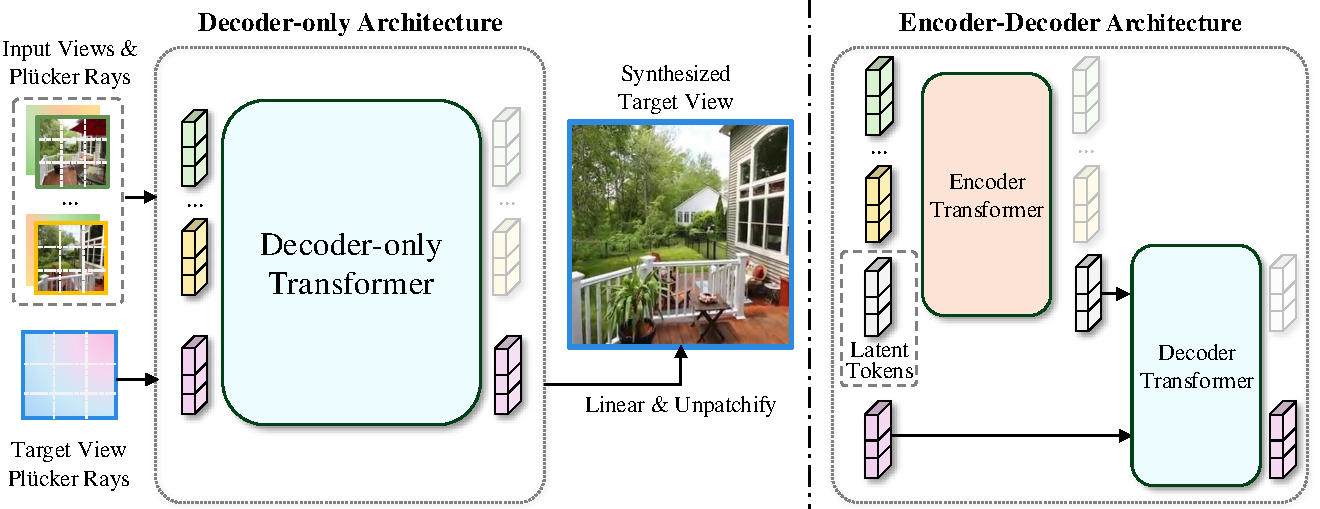
\includegraphics[width=\linewidth]{figures/model_3.pdf}
\vspace{-0.2in}
\caption{\small{
\textbf{\paperName{} model architecture.} \paperName{} first patchifies the posed input images into tokens. The target view to be synthesized is represented by its Pl\"ucker ray embeddings and is also tokenized. The input view and target tokens are sent to a full transformer-based model to predict tokens that are used to regress the target view pixels. We study two \paperName transformer architectures, a \textit{Decoder-only} architecture (left) and a \textit{Encoder-Decoder} architecture (right). 
}}
\vspace{-0.05in}
\label{fig: model}
\end{figure}


\paragraph{Framework.} As shown in Fig.~\ref{fig: model}, our \paperName method uses an end-to-end transformer model to directly render the target image. 
\paperName starts by tokenizing the input images. We first compute a pixel-wise Pl\"ucker ray embedding~\citep{plucker1865xvii} for each input view using the camera poses and intrinsics. 
We denote these Pl\"ucker ray embeddings as $\{\mathbf{P}_i \in \mathbb{R}^ {H\times W \times 6} | i = 1,\ldots,N\}$. We patchify the RGB images and Pl\"ucker ray embeddings into non-overlapping patches, following the image tokenization layer of ViT~\citep{dosovitskiy2020image}. We denote the image and Pl\"ucker ray patches of input image $\img_i$ as $\{\img_{ij} \in \mathbb{R}^{p\times p\times 3} | j = 1,\ldots,HW/p^2\}$ and $\{\mathbf{P}_{ij} \in \mathbb{R}^{p\times p\times 6}| j = 1,\ldots, HW/p^2\}$, respectively, where $p$ is the patch size. 
For each patch, we concatenate its image patch and Pl\"ucker ray embedding patch, reshape them into a 1D vector, and use a linear layer to map it into an input patch token 
$\mathbf{x}_{ij}$: 
\begin{align}
    \mathbf{x}_{ij} = \text{Linear}_\mathit{input}([\img_{ij}, \mathbf{P}_{ij}]) \in \mathbb{R}^d,
\end{align}
where $d$ is the latent size, and $[\cdot, \cdot]$ means concatenation.

Similarly, \paperName{} represents the target pose to be synthesized as its Pl\"ucker ray embeddings $\mathbf{P}^t \in \mathbb{R}^ {H\times W \times 6}$, computed from the given target extrinsics $\mathbf{E}^t$ and intrinsics $\mathbf{K}^t$. We use the same patchify method and another linear layer to map it to the Pl\"ucker ray tokens of the target view, denoted as:
\begin{align}
    \quad \mathbf{q}_{j} = \text{Linear}_\mathit{target}(\mathbf{P}^{t}_{j}) \in \mathbb{R}^d,
\end{align}
where $\mathbf{P}^{t}_{j}$ is the Pl\"ucker ray embedding of the $j^\text{th}$ patch in the target view.

We flatten the input tokens into a 1D token sequence, denoted as  $x_1, \ldots, x_{\mathit{l}_x}$, where $\mathit{l}_x\!=\!NHW/p^2$ is the sequence length of the input image tokens. We also flatten the target query tokens as $q_1, \ldots, q_{\mathit{l}_q}$ from the ray embeddings, with $\mathit{l}_q=HW/p^2$ as the sequence length. 

\paperName{} then synthesizes a novel view by conditioning on the input view tokens using a full transformer model $M$:
\begin{align}
    y_1, \ldots, y_\mathit{l_q} = M(q_1, \ldots, q_\mathit{l_q} | x_1, \ldots, x_\mathit{l_x}).
\end{align}
Specifically, the output token $y_j$ is an updated version of $q_j$, containing information for predicting the pixel values of the $j^{\text{th}}$ patch of the target view. More details of model $M$ are described in Sec.~\ref{sec:method_model_archs}.

We recover the spatial structure of output tokens using the inverse operation of the flatten operation. To regress RGB values of the target patch, we employ a linear layer followed by a sigmoid function:
\begin{align}
    \hat{\mathbf{I}}_{j}^t = \text{Sigmoid}{(\text{Linear}_{out}(y_{j}))} \in \mathbb{R}^{3p^2}.
\end{align}
We reshape the predicted RGB values back to the 2D patch in $\mathbb{R}^{p\times p \times 3}$, and then form the synthesized novel view $\hat{\mathbf{I}}^t$ by performing the same operation on all target patches independently.


\paragraph{Loss Function.}

Following prior works~\citep{zhang2024gslrmlargereconstructionmodel, hong2024lrmlargereconstructionmodel}, we train \paperName{} with photometric novel view rendering losses:
\begin{align}
    \mathcal{L} = \text{MSE}(\hat{\mathbf{I}}^t, \mathbf{I}^t) + \lambda \cdot \text{Perceptual}(\hat{\mathbf{I}}^t, \mathbf{I}^t),
\end{align}
where $\lambda$ is the weight for balancing the perceptual loss~\citep{johnson2016perceptual}.



\subsection{Transformer-Based Model Architecture}
\label{sec:method_model_archs}

In this subsection, we present two LVSM architectures---\textit{encoder-decoder} and \textit{decoder-only}---both designed to minimize 3D inductive biases.
Following their name, `\textit{encoder-decoder}' first converts input images to an intermediate latent representation before decoding the final image pixels, whereas `\textit{decoder-only}' directly outputs the synthesized target view without an intermediate representation, further minimizing inductive bias in its design. 
Unlike most standard language model transformers~\citep{vaswani2017transformer,jaegle2021perceiver, radford2019language}, which typically use full attention for encoders and causal/cross attention for decoders, we adopt dense \textbf{full self-attention} across all our encoder and decoder architectures. 
% \textit{\textbf{
The naming of our models is based on their output characteristics, instead of being strictly tied to the transformer architecture they utilize.
%}} 
Please refer to Appendix~\ref{appendix:naming_clarification} for a further detailed discussion of the naming. 



\paragraph{Encoder-Decoder Architecture.}
The encoder-decoder LVSM comes with a learned latent scene representation for view synthesis, avoiding the use of NeRF, 3DGS, and other representations.
The encoder first maps the input tokens to an intermediate 1D array of latent tokens (serving as a latent scene representation). The decoder then predicts the outputs, conditioning on the latent tokens and target pose.

Similar to the triplane tokens in LRMs~\citep{hong2024lrmlargereconstructionmodel,wei2024meshlrm}, we use $l$ learnable latent tokens $\{e_k \in \mathbb{R}^d \vert k=1, ..., l \}$ to aggregate information from input tokens $\{x_i\}$. The encoder, denoted as $\mathrm{Transformer}_\mathit{Enc}$, uses multiple transformer layers with self-attention. We concatenate $\{x_i\}$ and $\{e_k\}$ as the input to $\mathrm{Transformer}_\mathit{Enc}$, which performs information aggregation between them to update $\{e_k\}$. 
The output tokens that correspond to the latent tokens, denoted as $\{z_k\}$, are used as the intermediate latent scene representation. The other tokens (updated from $\{x_i\}$, denoted as $\{x'_i\}$) are unused and discarded.


The decoder uses multiple transformer layers with self-attention.
In detail, the inputs are the concatenation of the latent tokens $\{z_k\}$ and the target view query tokens $\{q_j\}$. 
By applying self-attention transformer layers over the input tokens, we get output tokens with the same sequence length as the input. 
The output tokens that corresponds to the target tokens $q_1, \ldots, q_\mathit{lq}$ are treated as final outputs $y_1, \ldots, y_\mathit{lq}$, and the other tokens (updated from $\{z_i\}$, denoted as $\{z'_i\}$) are unused.
This architecture can be formulated as:
\begin{align}
    x'_1, \ldots, x'_\mathit{l_x}, z_1, \ldots, z_\mathit{l}  & = \mathrm{Transformer}_\mathit{Enc} (x_1, \ldots, x_\mathit{l_x}, e_1, \ldots, e_\mathit{l}) \\
    z'_1, \ldots, z'_{l}, y_1, \ldots, y_\mathit{l_q} &= \mathrm{Transformer}_\mathit{Dec} (z_1, \ldots, z_{l}, q_1, \ldots, q_\mathit{l_q}).
\end{align}



\paragraph{Decoder-Only Architecture.} Our alternate, decoder-only model further eliminates the need for an intermediate scene representation. Its architecture is similar to the decoder in the encoder-decoder architecture but differs in inputs and model size.
We concatenate the two sequences of input tokens $\{x_i\}$ and target tokens $\{q_j\}$.
The final output $\{y_j\}$ is the decoder's corresponding output for the target tokens $\{q_j\}$. The other tokens (updated from $\{x_i\}$, denoted as $\{x'_i\}$) are unused and discarded. This architecture can be formulated as:
\begin{align}
    x'_1, \ldots, x'_\mathit{l_x}, y_1, \ldots, y_\mathit{l_q}  = \mathrm{Transformer}_\mathit{Dec\mbox{-}only} ( x_1, \ldots, x_\mathit{l_x}, q_1, \ldots, q_\mathit{l_q})
\end{align}
Here $\mathrm{Transformer}_\mathit{Dec\mbox{-}only}$ has multiple full self-attention transformer layers.
